\documentclass[12pt]{article}
\usepackage[utf8]{inputenc}
\usepackage[brazil]{babel}
\usepackage{amsmath, amssymb, array, bm, geometry, booktabs, siunitx, graphicx, colortbl, parskip, xcolor}
\usepackage{listings}
\usepackage{color}
\usepackage{float}
\usepackage{fancyhdr}
\usepackage{titlesec}
\usepackage{hyperref}
\usepackage{listings}

\setlength{\headheight}{14.5pt}
\addtolength{\topmargin}{-2.5pt}
\geometry{a4paper, total={6in, 9in}}




\definecolor{codegray}{gray}{0.9}
\lstset{
    backgroundcolor=\color{codegray},
    basicstyle=\ttfamily\footnotesize,
    frame=single,
    breaklines=true,
    captionpos=b,
    numbers=left,
    numberstyle=\tiny,
    language=Python
}

% Cabeçalho
\pagestyle{fancy}
\fancyhf{}
\rhead{UnB}
\lhead{Departamento de Ci\^encias Mec\^anicas}
\cfoot{\thepage}

\titleformat{\section}{\large\bfseries}{\thesection}{1em}{}

\begin{document}

% Capa
\begin{titlepage}
    \centering
    
\includegraphics[width=12cm]{img/unb_bandeira.png} \\
    \vspace{1cm}
    \textsc{\Large Universidade de Bras\'ilia} \\
    \textsc{Departamento de Ciências Mec\^anicas} \\
    \textsc{Programa de P\'os-Gradua\c{c}\~ao} \\
    \vfill
    {\Large\bfseries Programa 5} \\
    \vspace{0.5cm}
    {\Large\bfseries Solução de Problemas Lineares - Estudo de caso} \\
    \vspace{0.5cm}
    \textbf{Disciplina: M\'etodos Num\'ericos} \\
    Professor: Dr. Rafael Gabler Gontijo \\
    \vfill
    \textbf{Aluno: Eng. Lucas Wanick — Mestrando em Engenharia Mec\^anica} \\
    \vspace{0.5cm}
        \today \\
\end{titlepage}


\section{Introdução}
Este relatório apresenta a resolução de dois problemas de engenharia, apresenados em sala de aula e desenvolvidos como parte do Programa 5 da disciplina de Métodos Numéricos. O primeiro problema trata da determinação das concentrações em um sistema de reatores interligados, enquanto o segundo aborda a condução de calor unidimensional transiente com geração interna e resfriamento convectivo por escoamento externo.

Ambos os problemas foram resolvidos utilizando métodos numéricos apropriados, selecionados com base em suas características estruturais e propriedades de estabilidade. O código foi implementado em linguagem Python, com estrutura modular e foco em eficiência computacional e clareza dos resultados.

\section{Problema 1: Concentração nos Reatores}

\subsection{Formulação do Problema}

O sistema consiste em uma rede de cinco reatores interligados, com coeficientes de fluxo entre as unidades. O objetivo é determinar as concentrações estacionárias de um determinado componente químico em cada reator, a partir das equações de balanço de massa em regime permanente.

\subsection{Escolha do Método de Gauss-Seidel}

Devido à natureza da matriz dos coeficientes — esparsa, com predominância diagonal — o método iterativo de Gauss-Seidel foi escolhido para a resolução do sistema. Este método oferece simplicidade de implementação, convergência adequada para sistemas diagonais dominantes e permite controle explícito da precisão por meio do critério de parada.

\subsection{Esquema do Sistema}

A figura abaixo representa o esquema da rede de reatores conforme discutido em aula.

\begin{figure}[H]
    \centering
    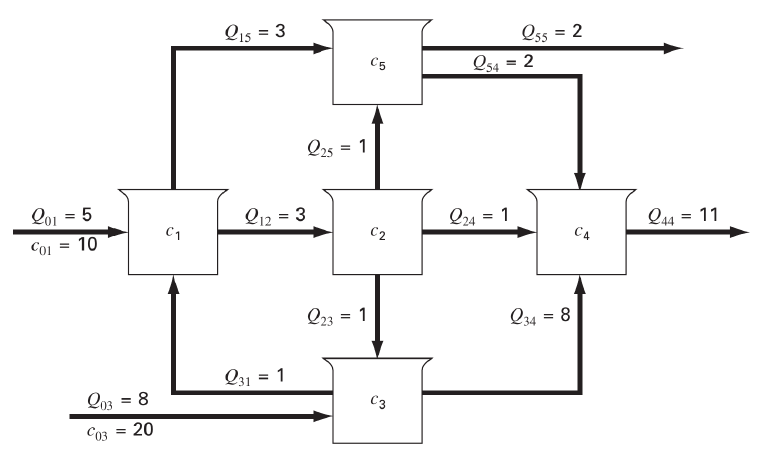
\includegraphics[width=0.8\textwidth]{img/figure1.png}
    \caption{Esquema da rede de reatores - Lousa de Aula}
\end{figure}

\subsection{Explicação Detalhada do Código}

O código implementa o método de Gauss-Seidel com controle de convergência via tolerância relativa. A matriz dos coeficientes e o vetor dos termos independentes são montados a partir dos dados fornecidos. O processo iterativo é conduzido até que a variação relativa das soluções entre iterações sucessivas caia abaixo da tolerância estipulada.

\begin{lstlisting}[language=Python, caption=Código - Resolução das concentrações]
# Montagem da matriz A e do vetor b
A = np.array([...])
b = np.array([...])

# Laco de Gauss-Seidel
x = np.zeros(len(b))
for iteration in range(max_iter):
    x_new = np.copy(x)
    for i in range(A.shape[0]):
        s1 = sum(A[i, j] * x_new[j] for j in range(i))
        s2 = sum(A[i, j] * x[j] for j in range(i + 1, A.shape[1]))
        x_new[i] = (b[i] - s1 - s2) / A[i, i]
    if np.all(np.abs(x_new - x) / np.abs(x_new + 1e-10) < tol):
        break
    x = x_new
\end{lstlisting}

\subsection{Resultados Numéricos e Interpretação Física}

As concentrações obtidas para cada reator indicam o equilíbrio das transferências de massa no sistema. O número de iterações necessário foi baixo, evidenciando a eficiência do método para este tipo de problema.

\section{Problema 2: Condução 1D Transiente com Geração}

\subsection{Formulação do Problema}

Considera-se um combustível sólido nuclear com geração volumétrica interna de calor e resfriamento convectivo em suas superfícies. A equação de condução transiente é resolvida para diferentes tempos, com o objetivo de analisar a evolução do perfil de temperatura ao longo da espessura da placa.

\begin{figure}[H]
    \centering
    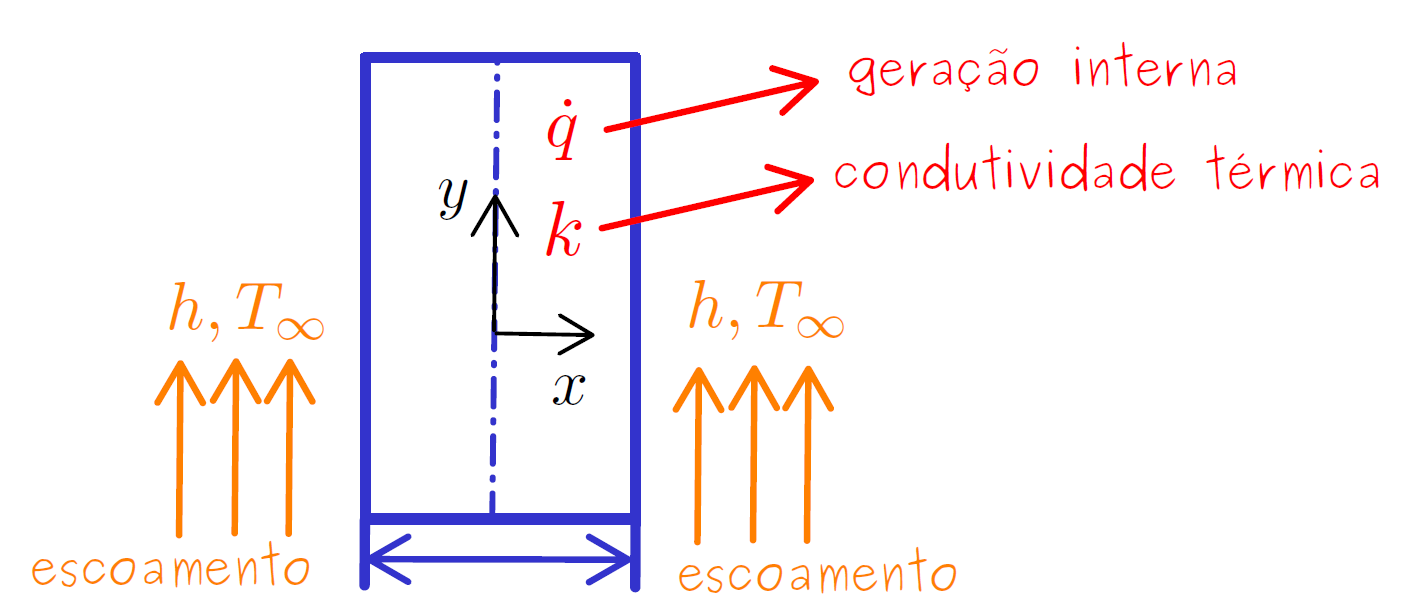
\includegraphics[width=0.8\textwidth]{img/figure2.png}
    \caption{Esquema combustível sólido com resfriamento - Lousa de Aula}
\end{figure}

\[
\frac{\partial T}{\partial t} = \alpha \nabla^2T + \frac{\dot{q}}{\rho c_p}
\]

Onde os dados fornecidos do exercício são:
\begin{align*}
    L = 10 mm , \hspace*{0.15cm} h = 1100 W/m^2 K , \hspace*{0.15cm} T_\infty=250^{\circ} C \\
    \dot{q}=10^7 W/m^3 , \hspace*{0.15cm} k=30 W/m K , \hspace*{0.15cm} \alpha = 5 \times 10^{-6} m^2/s
\end{align*}


\subsection{Justificativa da Escolha do Método de Thomas}

A discretização em diferenças finitas leva a um sistema linear tridiagonal a cada passo temporal. O método de Thomas (algoritmo de substituição para sistemas tridiagonais) é a escolha natural, por garantir eficiência \(\mathcal{O}(N)\) e estabilidade numérica elevada.

Assumindo:
\[
\boxed{Fo = \frac{\alpha \Delta t}{\Delta x^2}} \hspace*{0.3cm}
\text{;} \hspace*{0.3cm}
\boxed{Bi = \frac{h \Delta x}{k}} \hspace*{0.3cm}
\text{e} \hspace*{0.3cm}
\boxed{A = \frac{\dot{q} \Delta t}{\rho c_p}}
\]

e aplicando as condições de contorno, estruturamos uma matriz que descreve o comportamento do sistema nos nós internos, no centro como simétrico e à direita com convecção. O sistema linear assume o formato de:

\[
\begin{bmatrix}
1 + 2Fo   & -2Fo      & 0         & \cdots & 0 \\
-Fo       & 1 + 2Fo   & -Fo       & \cdots & 0 \\
0         & -Fo       & 1 + 2Fo   & -Fo    & 0 \\
\vdots    & \vdots    & \vdots    & \ddots & \vdots \\
0      & 0         & \cdots    & -2Fo    & 1 + 2Fo + 2Fo Bi
\end{bmatrix}
\cdot
\begin{bmatrix}
T_1^{P+1} \\
T_2^{P+1} \\
T_3^{P+1} \\
\vdots \\
T_n^{P+1}
\end{bmatrix}
=
\begin{bmatrix}
T_1^P + A \\
T_2^P + A \\
T_3^P + A \\
\vdots \\
T_n^P + Fo \left(2BiT_\infty + \frac{\dot{q}\Delta x^2}{k}\right)
\end{bmatrix}
\]

\subsection{Observação do Comportamento Temporal do Gradiente}

Os resultados mostram que o gradiente de temperatura evolui lentamente nos tempos iniciais, devido à inércia térmica do sistema. Nos tempos maiores, observa-se maior penetração térmica e estabilização do perfil.

\begin{figure}[H]
    \centering
    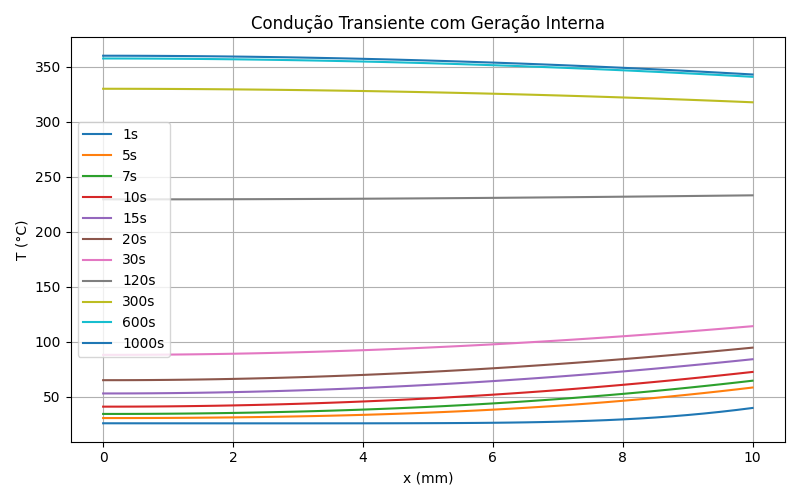
\includegraphics[width=0.8\textwidth]{img/Figure_3.png}
    \caption{Análise do perfil de condução transiente}
\end{figure}

\begin{figure}[H]
    \centering
    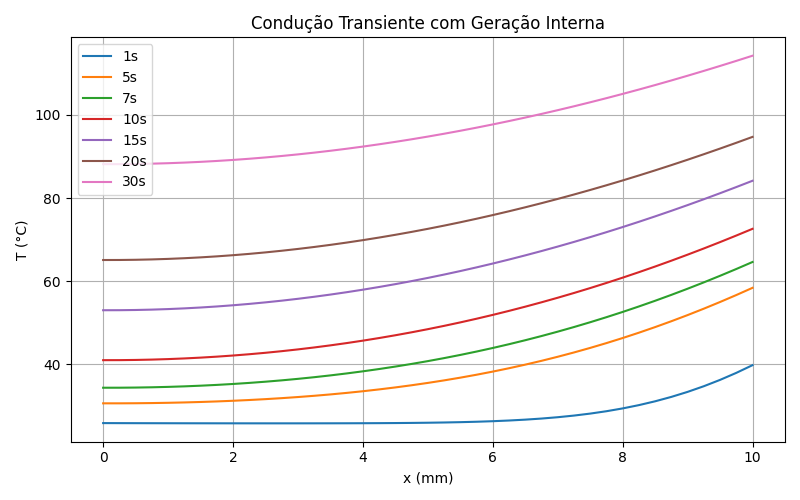
\includegraphics[width=0.8\textwidth]{img/Figure_4.png}
    \caption{Perfil de distribuição de temperatura para os tempos alvo solicitados}
\end{figure}

\subsection{Análise das Curvas em Tempos Maiores}

A análise das curvas em tempos superiores a 300 s revela a tendência de inflexão no perfil de temperatura, com aproximação progressiva ao regime permanente, caracterizado por um gradiente estabilizado.

\begin{figure}[H]
    \centering
    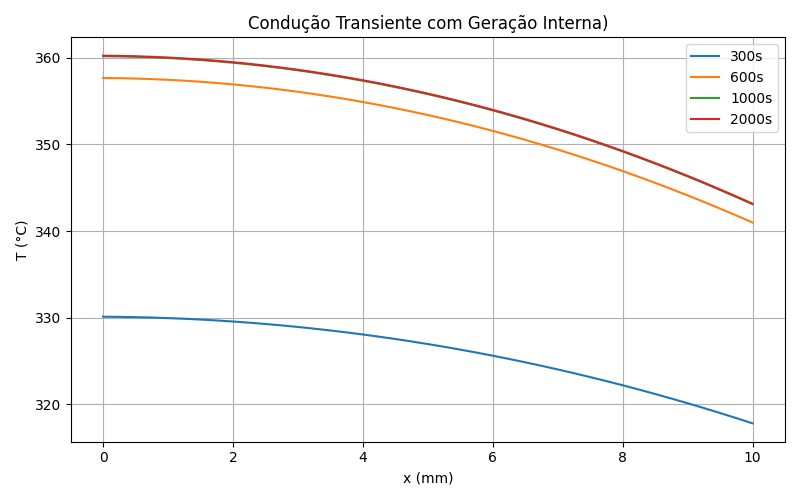
\includegraphics[width=0.8\textwidth]{img/Figure_6.png}
    \caption{Perfil de distribuição de temperatura no limite do regime permanente}
\end{figure}

Este comportamento se dá devido à condição inicial de temperatura, $T_0 = 25^\circ\mathrm{C}$, ser muito baixa e, apesar dos $10^7\,W/m^3$ da geração interna, temos um incremento máximo de temperatura de $\approx 3^\circ C$ à geração interna constante (estudo realizado alterando o parâmetro $T_\infty=25^\circ C$ para um tempo de 1 s), o que leva o escoamento a convectar muito mais calor para o sistema do que a variação gerada pela combustão do material, que possui propriedades em $\alpha = 5 \times 10^{-6} m^2/s$ muito pequeno, apesar de uma condutividade alta como a $k=30 W/m \cdot K$.

Em regime permanente, observa-se o equilíbrio entre geração interna e dissipação convectiva. A curva apresenta a característica típica de decaimento exponencial próximo às superfícies, com planalto central em função da geração constante.

\subsection{Justificativa do Método de Crank–Nicholson}

O método de Crank–Nicholson foi adotado por sua combinação de precisão (segundo ordem no tempo e no espaço) e estabilidade incondicional. Isso permite o uso de passos de tempo relativamente grandes sem comprometer a fidelidade da solução.

\subsection{Soluções de Otimização Implementadas}

Para otimização, foram implementados:
\begin{itemize}
    \item Controle adaptativo de convergência.
    \item Pré-computação dos coeficientes da matriz.
    \item Armazenamento seletivo dos \textit{snapshots} em tempos alvo.
\end{itemize}

\subsection{Validação da Solução com a Série Analítica}

Foi realizada uma comparação entre a solução numérica e a solução analítica por separação de variáveis no caso sem geração interna ($\dot{q} = 0$), com condição de contorno convectiva ($T_{\infty} = 250^\circ$C). Esta análise tem por objetivo isolar a contribuição do mecanismo de convecção no balanço energético, sem a influência do termo de geração volumétrica.

A Figura~\ref{fig:validacao_analitica} apresenta a comparação entre os perfis de temperatura obtidos numericamente e pela solução analítica, para os tempos de 5~s, 30~s, 120~s e 500~s. A Tabela~\ref{tab:erros_analitica} mostra os erros máximos observados em cada tempo.

Observa-se que nos primeiros tempos transientes, o erro entre as soluções é mais elevado, em função da dificuldade de convergência da série analítica truncada (número finito de termos) em representar variações abruptas de temperatura. Para tempos mais longos, o erro tende a diminuir, conforme esperado.

\begin{figure}[H]
    \centering
    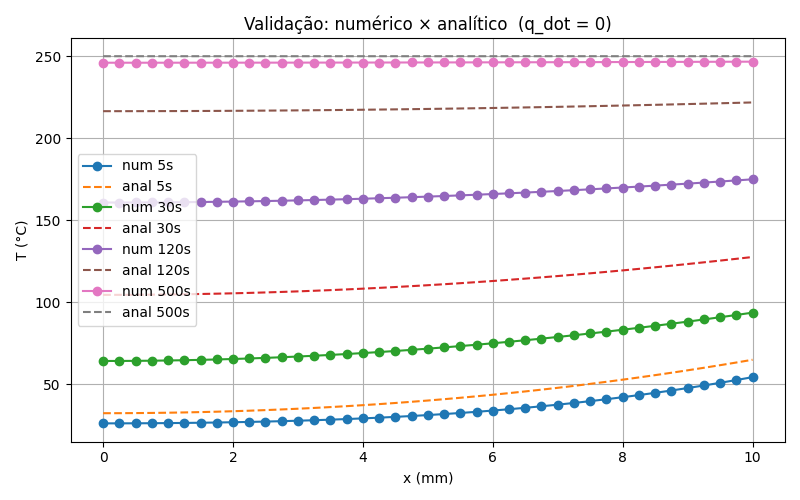
\includegraphics[width=0.8\textwidth]{img/Figure_5.png}
    \caption{Perfil de distribuição de temperatura no limite do regime permanente}
    \label{fig:validacao_analitica}
\end{figure}

\begin{table}[H]
    \centering
    \caption{Erros máximos observados entre solução numérica e analítica.}
    \label{tab:erros_analitica}
    \begin{tabular}{cc}
        \toprule
        Tempo [s] & Erro máximo [°C] \\
        \midrule
        5   & 10.803 \\
        30  & 40.267 \\
        120 & 55.640 \\
        500 & 3.964 \\
        \bottomrule
    \end{tabular}
\end{table}

\subsection{Explicação Detalhada do Código}

A função \texttt{run\_simulation} executa o avanço temporal com Crank–Nicholson, resolvendo o sistema tridiagonal em cada passo com o método de Thomas.

\begin{lstlisting}[language=Python, caption=Código - Solver da condução transiente]
def run_simulation(N, dt, qdot, tempos, Bi_eff, ...):
    dx = L / (N - 1)
    Fo = alpha * dt / dx**2
    T = np.full(N, T0)
    while t < tmax:
        Told = T.copy()
        # Montagem dos coeficientes tridiagonais
        a = np.full(N, -beta * Fo)
        b = np.full(N, 1 + 2 * beta * Fo)
        c = np.full(N, -beta * Fo)
        d = Told + (1 - beta) * Agen
        # Condicoes de contorno
        ...
        # Resolucao pelo metodo de Thomas
        T = thomas(a, b, c, d)
        ...
\end{lstlisting}

A função \texttt{theta\_series} permite a geração da solução analítica para comparação.

\section{Conclusões}

O Programa 5 permitiu consolidar conceitos fundamentais de solução de sistemas lineares e de equações diferenciais parciais. A escolha dos métodos numéricos foi fundamentada nas características estruturais de cada problema.

Observou-se que:
\begin{itemize}
    \item O método de Gauss-Seidel apresenta excelente desempenho para o sistema de reatores.
    \item O método de Thomas, aliado ao esquema de Crank–Nicholson, proporciona soluções estáveis e precisas para a condução transiente.
    \item A validação analítica reforçou a confiabilidade da implementação.
    \item O comportamento físico das soluções foi coerente com as expectativas teóricas.
\end{itemize}

O código modular desenvolvido serve como base para extensão a problemas mais complexos, com geometrias variadas e condições de contorno generalizadas.

\end{document}